\chapter{Objetivos}
\label{cap:capitulo3}
Una vez presentado el contexto general en el cual se enmarca el presente trabajo de fin de grado, en este capítulo se describen los objetivos y requisitos de este, así como la metodología y el plan de trabajo llevados a cabo.\\

\section{Descripción del problema}
\label{sec:descripcion}

La necesidad de implementar soluciones tecnológicas que automaticen y optimicen las tareas de recolección incrementando la eficiencia en la recolección, mejorando la calidad del producto y disminuyendo los costes asociados, surge debido a la situación actual de la agricultura en la que, uno de los mayores desafíos que enfrenta es la recolección de frutas y hortalizas, problema que deriva de la escasa mano de obra disponible y el proceso manual que esto conlleva, y de la posibilidad de que existan errores humanos en la identificación de los frutos para su recoleccción, pudiendo influenciar esto en la calidad del producto, especialmente en la recolección de frutos que requieren un manejo cuidadoso como las fresas.

La solución propuesta en este trabajo busca ayudar a mejorar esta situación,
proporcionando un robot de bajo coste y accesible para cualquier persona y que sirva para poder mejorar el proceso de reconocimiento por visión de la maduración de frutos, más concretamente fresas, para su posterior recolección. Por lo tanto, este proyecto pretende, como objetivo principal, utilizar un robot colaborativo que, gracias a su interfaz intuitiva y accesible para cualquier persona no acostumbrada a programar ni a la robótica, y junto con el sistema de detección elaborado con materiales de bajo coste, sea capaz de reconocer las fresas maduras de un sistema de cultivo agrícola vertical, para su posterior recolección por el brazo robótico gracias a la comunicación establecida entre el sistema de visión y el robot. 

Con el fin de alcanzar este objetivo principal, se han establecido los siguientes
subobjetivos:

\begin{enumerate}
  \item Investigar las soluciones actuales que cumplen con las características y objetivos establecidos.
  \item Seleccionar la técnica de inteligencia artificial de reconocimiento de frutas y seleccionar los componentes hardware necesarios para desarrollar el sistema de visión de bajo coste.
  \item Optimizar la técnica escogida y adaptarla de tal manera que sea capaz de funcionar en nuestra plataforma. Al ser una técnica basada en Machine Learning, se deberá crear un dataset de valor con imágenes de fresas y, por lo tanto, hacer un correcto tratamiento de los datos para conseguir un resultado preciso en el posterior entrenamiento.
  \item Realizar el entrenamiento con varios algoritmos de Machine Learning de
clasificación. Estudiar el rendimiento y precisión de cada uno de ellos a través de pruebas con el sistema de visión y fresas reales.
  \item Seleccionar el protocolo de comunicación entre el sistema de visión y el robot y llevar a cabo pruebas tanto simuladas a través del simulador que facilita el fabricante del robot como reales para establecer esta comunicación.
  \item Programación tanto del robot como del archivo en python que posee el código del sistema de reconocimiento de las fresas y el guardado de las posiciones y la distancia de estas a la posición de la cámara para su posterior envío al brazo robótico.
  \item Realización de pruebas de la aplicación final tanto en entornos simulados como reales.
\end{enumerate} 


\section{Requisitos}
\label{sec:requisitos}

Para solucionar los problemas descritos, además de cumplir los subobjetivos
marcados, este trabajo deberá cumplir los siguientes requisitos:

\begin{enumerate}
  \item Se utilizará \textit{GNU/Linux}, con la distribución \textit{Ubuntu 22.04 LTS} como sistema operativo en el hardware que se encargará de ejecutar el programa del sistema de visión.
  \item Los modelos entrenados se deben ajustar a las limitaciones hardware que ejecutará el programa del sistema de visión.
  \item El sistema deberá poder ser utilizado en tiempo real. 
  \item El \textit{hardware} utilizado para el desarrollo del sistema de visión debe ser lo suficientemente económico para ser adquirido por cualquier estudiante.
  \item La aplicación debe ser fácilmente reproducible y desplegable tanto en un entorno simulado como en un ambiente educativo real o de laboratorio.
\end{enumerate}  

\section{Competencias}
\label{sec:competencias}

Las competencias empleadas del grado, que han sido tomadas de las distintas asignaturas del mismo, y que han sido utilizadas para la realización de este proyecto se dividen tanto en generales como específicas, y son las siguientes:

\begin{enumerate} 
  \item \textit{Capacidad de organización y planificación: CG02.} Esta competencia ha sido empleada en la consecución de todo el trabajo de fin de grado, y queda reflejada tanto en las reuniones semanales o quincenales con el tutor responsable de este trabajo como en la wiki de GitHub \footnote{\url{https://github.com/RoboticsURJC/tfg-dcampoamor/wiki}} dedicada al proyecto, que refleja los avances y la organizacización llevada a cabo.  
  \item \textit{Conocimiento de una lengua extranjera: CG04.} Esta competencia ha sido utilizada a la hora de buscar toda clase de información para poder elaborar este proyecto, ya que se han utilizado documentos publicados en, al menos, una lengua extranjera, como lo es el inglés.
  \item \textit{Resolución de problemas: CG06.} Dado el nivel de conocimiento necesario en ciertas materias como la inteligencia artificial o la visión artificial, ha sido empleada para poder resolver los diversos inconvenientas que afrontar las pruebas prácticas relacionadas con estas áreas del trabajo suponían.
  \item \textit{Uso de internet como medio de comunicación y como fuente de información: CG21.} Para poder elaborar este trabajo de fin de grado, ha sido necesario emplear esta competencia para buscar la información necesaria y poder completar principalmente los capítulos 1 y 2.
  \item \textit{Conocimientos de informática relativos al ámbito de estudio: CG24.} Esta competencia ha sido empleada a la hora de desarrollar y programar la aplicación sobre la que trata este trabajo.
  \item \textit{Conocimientos básicos sobre el uso y programación de los ordenadores, sistemas operativos, bases de datos y programas informáticos con aplicación en ingeniería: CE3.} Para poder desarrollar la aplicación se tuvo que emplear esta competencia a la hora de llevar a cabo la partición del disco duro en el ordenador y poder instalar la versión de \textit{Ubuntu 22.04.5 LTS (Jammy Jellyfish)}.  
  \item \textit{Conocimientos sobre los fundamentos de automatismos y métodos de control: CE13.} Esta competencia se refleja en la programación de la toma de decisiones automática, donde el sistema ajusta las operaciones en función de los resultados obtenidos del sistema de visión, así como el trabajo sincronizado de varios dispositivos (cámara y robot) y la comunicación entre estos.
  \item \textit{Conocimiento de los principios de regulación automática y su aplicación a la automatización industrial: CE32.} Esta competencia se emplea una vez que el sistema de visión identifica el grado de maduración de la fresa, ya que el sistema toma la decisión de recolectar o no el fruto, ajustando los actuadores o robots para realizar la tarea de forma precisa, dependiendo de las condiciones detectadas. Así mismo, se emplea la regulación automática en la optimización del proceso ajustando el comportamiento del robot en función del estado de la maduración de la fresa, maximizando la velocidad de la aplicación y su precisión.
  \item \textit{Capacidad para diseñar sistemas de control y automatización industrial: CE33.} Gracias a esta competencia se ha podido estructurar el sistema completo, incluyendo la parte de visión artificial, el procesamiento de imágenes, la toma de decisiones y el control del brazo robótico, integrando todos los datos en tiempo real y llevando a cabo operaciones de monitoreo y seguimiento de la aplicación y sus operaciones en remoto, tal y como se realizó en la etapa de pruebas.
  
\end{enumerate}  

Por otro lado, las competencias adquiridas con el desarrollo de este trabajo fin de grado, y que aparecen descritas en la guía docente de la propia asignatura, son las siguientes:

\begin{enumerate}
  \item \textit{Capacidad de análisis y síntesis: CG01.} Esta competencia se adquiere debido a la necesidad de la búsqueda y recopilación de información necesaria para el desarrollo del proyecto.
  \item \textit{Razonamiento crítico: CG11.} En relación con la competencia adquirida CG01, el razonamiento crítico se emplea a la hora de filtrar, seleccionar y decidir qué de toda la información obtenida es válido, cómo se puede utilizar y cómo ajustarlo y añadirlo al contenido del proyecto.
  \item \textit{Aprendizaje autónomo: CG13.} Esta competencia ha sido adquirida dada  la necesidad de adaptarse al marco técnico en cuál se desarrolla este proyecto, su complejidad, y la constante actualización y mejoras de las técnicas que pueden ser empleadas para el desarrollo del mismo.
  \item \textit{Adaptación a nuevas situaciones: CG14.} Esta competencia se adquiere gracias a la aplicación de la competencia adquirida \textit{CG13 Aprendizaje autónomo}, justificada anteriormente, y que se puede ver reflejada en el proyecto.
  \item \textit{Capacidad de aplicar los conocimientos teóricos en la práctica: CG20.} La parte empírica y práctica del proyecto refleja la adquisición de esta competencia.
  \item \textit{Capacidad para entender el lenguaje y propuestas de otros especialistas: CG22.} Esta competencia se ha visto reflejadan dado que, en relación con el resto de competencias adquiridas, sobre todo con las competencias \textit{CG01 Capacidad de análisis y síntesis} y \textit{CG11 Razonamiento crítico}, se ha tenido la necesidad de consulta, recopilación y filtrado de información y metodologías científicas existentes para poder desarrollar la aplicación del proyecto.
\end{enumerate} 


\section{Metodología}
\label{sec:metodologia}

Para lograr los objetivos descritos anteriormente, se optó por emplear el método DMADV (Definir, Medir, Analizar, Diseñar,Verificar), perteneciente a la metodología \textit{Six Sigma} (ver en Figura \ref{fig:DMADV}). 

Se decidió optar por esta metodología dado que la aplicación desarrollada en este trabajo está basada en otros proyectos y estudios similares ya existentes, y esta metodología está diseñada para desarrollar procesos o productos nuevos o significativamente mejorados, independientemente de si partes de cero o si te basas en conocimientos previos, y esta información recopilada fue utilizada como punto de partida en las fases iniciales de la metodología. A continuación, se detallan las fases del método DMADV y cómo han sido aplicadas en el desarrollo de este proyecto.

\begin{itemize}
  \item Definir: En esta fase se establecen como objetivos del proyecto la identificación de fresas maduras mediante un sistema de visión artificial y su integración con el brazo robótico encargado de su recolección. 
  \item Medir: Tomando como referencia el estado del arte existente, se llevó a cabo la selección de la tecnología (hardware y software necesarios) y las métricas existentes para poder considerar que las detecciones son aceptables y suficientes, basándose así el trabajo en proyectos y estudios que han demostrado ser eficaces, constituyendo un proyecto robusto y eficiente y ayudando a evitar problemas comunes ya que se sostiene sobre conocimientos adquiridos de proyectos similares testados. 
  \item Analizar: En esta etapa se llevaron a cabo pruebas con diferentes algoritmos y sistemas para detección de objetos, tanto en imágenes como en vídeo a tiempo real, para poder determinar cuál ofrecía un mejor rendimiento en precisión y velocidad y se ajustaba a los requisitos que presentaba el hardware disponible para el desarrollo del proyecto.  
  \item Diseñar: En base a los resultados obtenidos en la fase de análisis, se configuró el sistema de reconocimiento por visión incluyendo el hardware, previamente seleccionado, y el software, compuesto por los códigos y entornos necesarios para poder desarrollarlo y ejecutarlo, y su integración con el robot.
  \item Verificar: Finalmente, se llevaron a cabo pruebas para verificar que el sistema funcionaba y cumplía con los requisitos definidos, validándose la precisión en la identificación de las fresas maduras con distintas intensidades de luz ambiente y la comunicación y el correcto funcionamiento del brazo robótico.
\end{itemize}
  
\begin{figure} [H]
    \begin{center}
      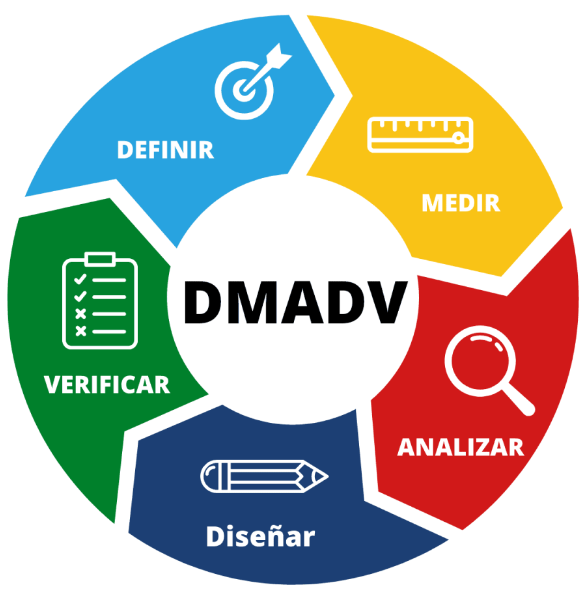
\includegraphics[width=9cm]{figs/DMADV.png}
    \end{center}
    \caption{Ciclo de la metodología DMADV}
    \label{fig:DMADV}
\end{figure}

	
\section{Plan de trabajo}
\label{sec:plantrabajo}
El desarrollo y seguimiento que el proyecto ha seguido es una planificación en base a reuniones semanales con el tutor, en las cuales se revisaron los avances, se fijaron nuevos objetivos y se discutieron y propusieron posibles mejoras, mientras que el trabajo se organizó en varias fases clave: 
\begin{enumerate}
  \item \textit{Investigación inicial:} En esta fase, se investigó el estado del arte relacionado con sistemas de visión artificial y técnicas de reconocimiento de objetos, especialmente aplicadas a la maduración de frutas y hortalizas, y utilizando para ello artículos científicos, capítulos de libros y proyectos previos. 
  \item \textit{Diseño y desarrollo del sistema de visión artificial:} Esta fase se centró en el diseño y la implementación del sistema de visión artificial, abarcando tanto el desarrollo del software como la integración del hardware, e incluyendo la calibración y obtención de los parámetros intrínsecos a la cámara y las diversas pruebas realizadas con distintos sistemas y códigos, hasta seleccionar el \textit{software} funcional con el que se llevó a cabo el proyecto finalmente.
  \item \textit{Pruebas en entorno simulado:} Durante esta fase se realizaron múltiples pruebas y ajustes para optimizar el funcionamiento del sistema y comprobar su funcionamiento en diferentes escenarios, simulando de manera separada la programación del robot, para el que se utilizó un simulador en una máquina virtual, y la detección y funcionamiento del sistema de visión, cuyos algoritmos se afinaron para mejorar la precisión en la detección y se ajustaron los parámetros relacionados con la cámara en los códigos para poder obtener las coordenadas y distancia real de las detecciones respecto a la cámara y poder transmitirselas al brazo robótico. Finalmente, también se llevaron a cabo pruebas de comunicación entre el sistema de visión y el robot, poniendo a prueba su programación, para que este alcanzase el punto de la detección.
  \item \textit{Pruebas en entorno real:} Una vez desarrollado el prototipo inicial, el sistema completo fue sometido a pruebas en un entorno real de lo que sería la aplicación final. 
  \item \textit{Escritura de la memoria:} Con el sistema ya afinado y probado, se procedió a la redacción de la memoria del proyecto. En esta etapa, se documentó detalladamente todo el proceso seguido, desde la investigación inicial hasta los resultados finales obtenidos durante las pruebas reales. 
\end{enumerate}
\pagebreak
Todo el contenido del proyecto se puede encontrar en un repositorio público de GitHub \footnote{\url{https://github.com/RoboticsURJC/tfg-dcampoamor}}, donde en el apartado Wiki \footnote{\url{https://github.com/RoboticsURJC/tfg-dcampoamor/wiki}} de dicho repositorio puede verse el desarrollo del trabajo en semanas a lo largo de los meses, durante el trascurso del proyecto.\\
\\
\\
\\
Después de haber revisado los objetivos, requisitos, competencias, metodología y el plan de trabajo implementado para la realización de este proyecto, se abordarán las plataformas de desarrollo empleadas.

